\let\negmedspace\undefined
\let\negthickspace\undefined
\documentclass[journal,12pt,onecolumn]{IEEEtran}
\usepackage{cite}
\usepackage{amsmath,amssymb,amsfonts,amsthm}
\usepackage{algorithmic}
\usepackage[version=4]{mhchem}
\usepackage{graphicx}
\usepackage{textcomp}
\usepackage{xcolor}
\usepackage{amsmath}
\usepackage{txfonts}
\usepackage{listings}
\usepackage{enumitem}
\usepackage{mathtools}
\usepackage{gensymb}
\usepackage{comment}
\usepackage[breaklinks=true]{hyperref}
\usepackage{tkz-euclide} 
\usepackage{gvv}                                        
%\def\inputGnumericTable{}                                 
\usepackage[latin1]{inputenc}     
\usepackage{xparse}
\usepackage{color}                                            
\usepackage{array}                                            
\usepackage{longtable}                                       
\usepackage{calc}                                             
\usepackage{multirow}
\usepackage{multicol}
\usepackage{hhline}                                           
\usepackage{ifthen}                                           
\usepackage{lscape}
\usepackage{tabularx}
\usepackage{array}
\usepackage{float}
\newtheorem{theorem}{Theorem}[section]
\newtheorem{problem}{Problem}
\newtheorem{proposition}{Proposition}[section]
\newtheorem{lemma}{Lemma}[section]
\newtheorem{corollary}[theorem]{Corollary}
\newtheorem{example}{Example}[section]
\newtheorem{definition}[problem]{Definition}
\newcommand{\BEQA}{\begin{eqnarray}}
\newcommand{\EEQA}{\end{eqnarray}}
\newcommand{\define}{\stackrel{\triangle}{=}}
\theoremstyle{remark}
\newtheorem{rem}{Remark}
% Marks the beginning of the document
\begin{document}
\title{gg Gate 2023}
\author{ai25btech11014-Gooty Suhas}
\maketitle

\section*{General Aptitude (GA)}
\vspace{0.5cm}
\begin{enumerate}

\item The village was nestled in a green spot,\underline{\hspace{10mm}} the ocean and the hills.
\begin{enumerate}
\item through
\item in
\item at
\item between
\end{enumerate}
\vspace{0.5cm}

\item Disagree : Protest :: Agree : \underline{\hspace{10mm}}(By word meaning)
\begin{enumerate}
\item Refuse
\item Pretext
\item Recommend
\item Refute
\end{enumerate}
\vspace{0.5cm}

\item A 'frabjous' number is defined as a 3-digit number with all digits odd, and no two adjacent digits being the same. For example, 137 is a frabjous number, while 133 is not. How many such frabjous numbers exist?
\begin{enumerate}
\item 125
\item 720
\item 60
\item 80
\end{enumerate}
\vspace{0.5cm}

\item Which one among the following statements must be TRUE about the mean and the median of the scores of all candidates appearing for GATE 2023?
\begin{enumerate}
\item The median is at least as large as the mean.
\item The mean is at least as large as the median.
\item At most half the candidates have a score that is larger than the median.
\item At most half the candidates have a score that is larger than the mean.
\end{enumerate}
\vspace{0.5cm}

\item In the given diagram, ovals are marked at different heights (h) of a hill. Which one of the following options P, Q, R, and S depicts the top view of the hill?

\begin{figure}[H]
    \centering
    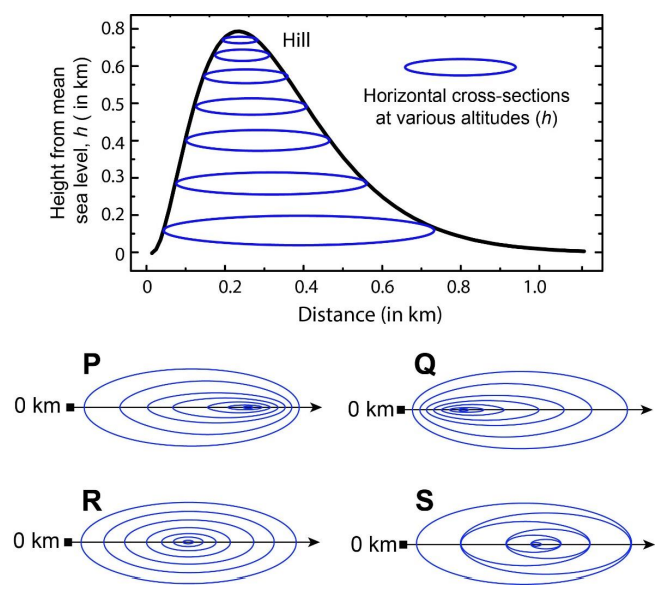
\includegraphics[width=0.8\textwidth]{figs/fig1.png}
    \caption{Image for questions 5}
    \label{fig:question5}
\end{figure}
\vspace{0.5cm}



\begin{enumerate}
\item P
\item Q
\item R
\item S
\end{enumerate}
\vspace{0.5cm}

\item Residency is a famous housing complex with many well-established individuals among its residents. A recent survey conducted among the residents of the complex revealed that all of those residents who are well established in their respective fields happen to be academicians. The survey also revealed that most of these academicians are authors of some best-selling books. Based only on the information provided above, which one of the following statements can be logically inferred with certainty?
\begin{enumerate}
\item Some residents of the complex who are well established in their fields are also authors of some best-selling books.
\item All academicians residing in the complex are well established in their fields.
\item Some authors of best-selling books are residents of the complex who are well established in their fields.
\item Some academicians residing in the complex are well established in their fields.
\end{enumerate}
\vspace{0.5cm}

\item Ankita has to climb 5 stairs starting at the ground, while respecting the following rules:  \\
1. At any stage, Ankita can move either one or two stairs up.  \\
2. At any stage, Ankita cannot move to a lower step.\\  
Let F(N) denote the number of possible ways in which Ankita can reach the Nth stair. For example, F(1) = 1, F(2) = 2, F(3) = 3.\\
The value of F(5) is \underline{\hspace{10mm}}
\begin{enumerate}
\item 8
\item 7
\item 6
\item 5
\end{enumerate}
\vspace{0.5cm}

\item The information contained in DNA is used to synthesize proteins that are necessary for the functioning of life. DNA is composed of four nucleotides: Adenine (A), Thymine (T), Cytosine (C), and Guanine (G). The information contained in DNA can then be thought of as a sequence of these four nucleotides: A, T, C, and G. DNA has coding and non-coding regions. Coding regions--where the sequence of these nucleotides are read in groups of three to produce individual amino acids--constitute only about 2\% of human DNA. For example, the triplet of nucleotides CCG codes for the amino acid glycine, while the triplet GGA codes for the amino acid proline. Multiple amino acids are then assembled to form a protein. Based only on the information provided above, which of the following statements can be logically inferred with certainty?
\begin{enumerate}
\item only (i)
\item only (ii)
\item both (i) and (ii)
\item neither (i) nor (ii)
\end{enumerate}
\vspace{0.5cm}

\item Which one of the given figures P, Q, R and S represents the graph of the following function?  
$f(x) = \left|\,|x+2| - |x-1|\,\right|$

\begin{figure}[H]
    \centering
    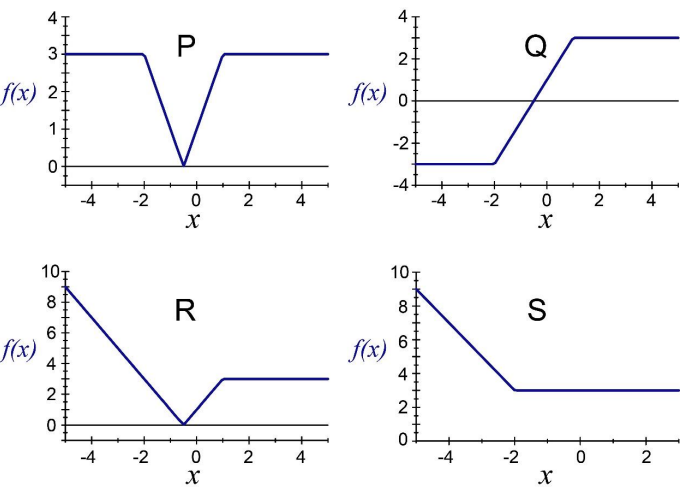
\includegraphics[width=0.8\textwidth]{figs/fig2.png}
    \caption{Image for questions 9}
    \label{fig:question9}
\end{figure}
\vspace{0.5cm}




\begin{enumerate}
\item P
\item Q
\item R
\item S
\end{enumerate}
\vspace{0.5cm}

\item An opaque cylinder is suspended in the path of a parallel beam of light, such that its shadow is cast on a screen oriented perpendicular to the direction of the light beam. The cylinder can be reoriented in any direction within the light beam. Under these conditions, which one of the shadows P, Q, R, and S is NOT possible?

\begin{figure}[H]
    \centering
    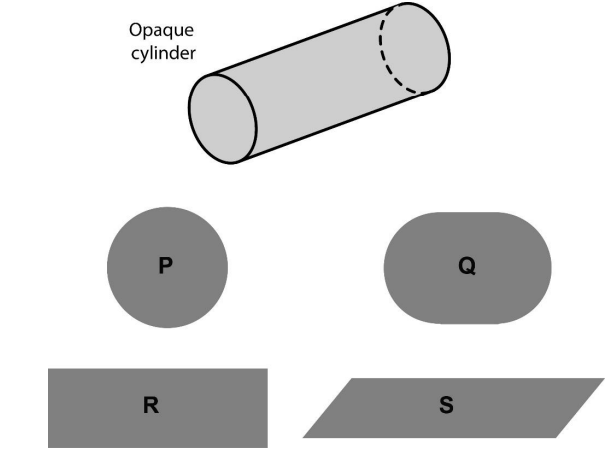
\includegraphics[width=0.8\textwidth]{figs/fig3.png}
    \caption{Image for questions 10}
    \label{fig:question10}
\end{figure}
\vspace{0.5cm}






\begin{enumerate}
\item P
\item Q
\item R
\item S
\end{enumerate}
\vspace{0.5cm}
\newpage
\section*{PART A: COMPULSORY SECTION FOR ALL CANDIDATES}
\vspace{0.5cm}


\item Which of the following is a chronostratigraphic unit?
\begin{enumerate}
\item Member
\item Stage
\item Acme Zone
\item Period
\end{enumerate}
\vspace{0.5cm}

\item During contact metamorphism, with increasing temperature,
\begin{enumerate}
\item the ratio of volume to surface area of mineral grains increases.
\item the ratio of volume to surface area of mineral grains decreases.
\item the reaction kinetics becomes slower.
\item hydrous minerals become more stable.
\end{enumerate}
\vspace{0.5cm}

\item The dimension of dynamic viscosity is
\begin{enumerate}
\item MIL$^{-1}$T$^{-2}$
\item MIL$^{-1}$T$^{-1}$
\item M$^{0}$L$^{2}$T$^{-1}$
\item M$^{0}$L$^{0}$T$^{0}$
\end{enumerate}
\vspace{0.5cm}

\item At a depth of about 400 km inside the Earth, which one of the following occurs?
\begin{enumerate}
\item Conversion of most silicates to perovskite structure
\item Conversion of plagioclase-peridotite to spinel-peridotite
\item Transformation of olivine to spinel structure
\item Conversion of spinel-peridotite to plagioclase-peridotite
\end{enumerate}
\vspace{0.5cm}

\item Equatorial radius of which one of the following planets is closest to that of the Earth?
\begin{enumerate}
\item Mercury
\item Venus
\item Mars
\item Neptune
\end{enumerate}
\vspace{0.5cm}


\item Variation of Bouguer anomaly obtained along a profile after applying all the necessary corrections is due to
\begin{enumerate}
\item topographic undulation above the datum plane.
\item increase in densities of crustal rocks with depth.
\item lateral density variations.
\item vertical density contrast across Moho.
\end{enumerate}
\vspace{0.5cm}

\item The heat production (Q$_r$) of a granitic rock due to decay of the radioactive elements U, Th and K having concentration C$_u$, C$_{Th}$, and C$_K$, respectively, is given by the expression Q$_r$ = $\alpha$C$_u$ + $\beta$C$_{Th}$ + $\gamma$C$_K$. Which one of the following correctly represents the relation between the magnitude of coefficients $\alpha$, $\beta$, $\gamma$ (in $\mu$Wkg$^{-1}$)?
\begin{enumerate}
\item $\alpha > \beta > \gamma$
\item $\alpha < \beta > \gamma$
\item $\alpha > \beta \gamma$
\item $\alpha < \beta < \gamma$
\end{enumerate}
\vspace{0.5cm}

\item Which one of the following Phanerozoic periods has the shortest duration of time?
\begin{enumerate}
\item Cambrian
\item Devonian
\item Cretaceous
\item Silurian
\end{enumerate}

\item Based on the given mineral proportions, which one of the following statements is CORRECT?\\
Rock\\
Mineral Proportion\\
X Olivine : Orthopyroxene : Clinopyroxene :: 50 : 30 : 20\\
Y Plagioclase : Alkali feldspar : Quartz :: 25 : 45 : 30\\
Z Biotite : Plagioclase : Alkali feldspar : Quartz :: 20 : 25 : 35 : 20
\begin{enumerate}
\item Y is more felsic compared to X -- Z
\item X is more felsic compared to Y -- Z
\item Z is more felsic compared to X -- Y
\item Y is the most felsic and Z is the most mafic
\end{enumerate}

\item The CORRECT sequence(s) of electromagnetic radiations in terms of increasing wavelength is/are
\begin{enumerate}

\item Gamma ray $<$ UV $<$ Near--IR
\item X--ray $<$ Visible light $<$ Thermal IR
\item Microwave $<$ Visible light $<$ Radio wave
\item Microwave $<$ Thermal IR $<$ Near--IR
\end{enumerate}

\item Which of the given folds is/are represented by the stereoplot?

\begin{figure}[H]
    \centering
    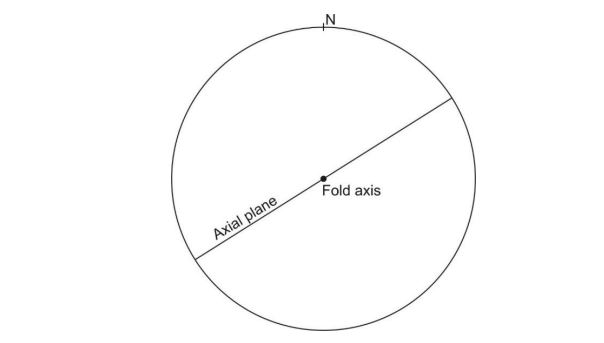
\includegraphics[width=0.6\textwidth]{figs/fig4.png}
    \caption{Image for questions 21}
    \label{fig:question21}
\end{figure}
\vspace{0.5cm}


\begin{enumerate}
\item Horizontal fold
\item Vertical fold
\item Upright fold
\item Recumbent fold
\end{enumerate}
\vspace{0.5cm}




\item The bulk density and water content of a soil are 1800 kg/m$^3$ and 18\%, respectively. The dry density of the soil calculated from the given information is \underline{\hspace{10mm}} kg/m$^3$.
\vspace{0.5cm}

\item In a seismic reflection survey over a two--layered Earth model having densities and seismic velocities $\rho_1$ = 2000 kg/m$^3$, $V_1$ = 1800 m/s for the first layer and $\rho_2$ = 3000 kg/m$^3$, $V_2$ = 2100 m/s for the second layer, the normal incidence P--wave reflection coefficient is \underline{\hspace{10mm}}.
\vspace{0.5cm}

\item The resistivity of a rock, 100\% saturated with water of resistivity 0.25 $\Omega$m, is 60 $\Omega$m. Assuming tortuosity and cementation exponents to be 1 and 2, respectively, the porosity of the rock is \underline{\hspace{10mm}}\%
\vspace{0.5cm}

\item Let us consider that a student misses cancelling the self--potential between potential electrodes before injecting current into the subsurface, in a Wenner electrical resistivity survey using DC resistivity meter over a horizontally stratified Earth. In direct and reverse modes of measurement (when current flows from C1 to C2 and C2 to C1, respectively) with the same magnitude of current flow, the potential differences recorded are +158 mV and --214 mV, respectively. The self--potential between the potential electrodes before injecting current was \underline{\hspace{10mm}} mV.
\vspace{0.5cm}


\item For the given figure, considering Pratt's model of isostatic compensation at the crust--mantle boundary, the crustal density ($\rho_1$) that explains 1.5 km deep lake is \underline{\hspace{10mm}} kg/m$^3$. (Consider density of water $\rho_w$ = 1000 kg/m$^3$)

\begin{figure}[H]
    \centering
    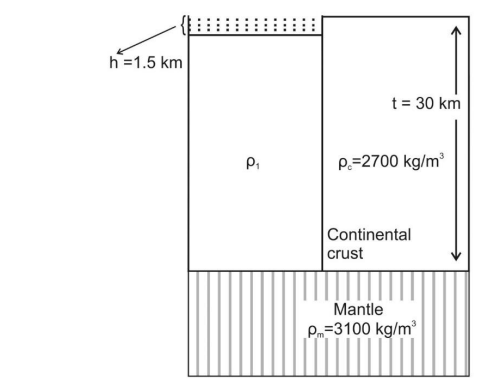
\includegraphics[width=0.7\textwidth]{figs/fig5.png}
    \caption{Image for questions 26}
    \label{fig:question26}
\end{figure}
\vspace{0.5cm}


\vspace{0.5cm}

\newpage
\section*{PART B (SECTION 1): FOR GEOLOGY CANDIDATES ONLY}
\vspace{0.5cm}

\item Which one of the following mineral pairs shows solid solubility through coupled substitution of elements?
\begin{enumerate}
\item Albite -- Anorthite
\item Albite -- Orthoclase
\item Grossular -- Andradite
\item Jadeite -- Aegirine
\end{enumerate}
\vspace{0.5cm}

\item The behavior of trace elements in magmatic systems follows
\begin{enumerate}
\item Henry's Law
\item Raoult's Law
\item Fick's Second Law
\item First Law of Thermodynamics
\end{enumerate}
\vspace{0.5cm}



\item \parbox[t]{\linewidth}{Choose the CORRECT statement regarding crystallization of a single feldspar of composition Or$_{50}$Ab$_{50}$ in the Albite--Orthoclase system.}
\begin{enumerate}
\item The mineral can form in hypersolvus but not in subsolvus feldspar system.
\item The mineral can form in subsolvus but not in hypersolvus feldspar system.
\item The mineral can crystallize in both hypersolvus and subsolvus feldspar system.
\item The mineral can crystallize neither in hypersolvus nor in subsolvus feldspar system.
\end{enumerate}
\vspace{0.5cm}

\item Given $\Delta V_r$ and $\Delta S_r$ are the volume and entropy of reaction, respectively, the most suitable conditions for the reaction to be used as a geothermometer are
\begin{enumerate}
\item small $\Delta V_r$, but large $\Delta S_r$
\item small $\Delta S_r$, but large $\Delta V_r$
\item positive $\Delta V_r$, but negative $\Delta S_r$
\item negative $\Delta V_r$ but positive $\Delta S_r$
\end{enumerate}
\vspace{0.5cm}

\item In which one of the given mass extinction events, global cooling that resulted in glaciation and lowering of sea level, is considered as major cause of extinction for more than 50\% of marine fauna?
\begin{enumerate}
\item Cretaceous -- Paleogene
\item Permian -- Triassic
\item Ordovician -- Silurian
\item Holocene
\end{enumerate}
\vspace{0.5cm}

\item Processes of fossilization affecting an organism from its death to burial under sediments come under the study of
\begin{enumerate}
\item Biostratinomy
\item Biostratigraphy
\item Taphonomy
\item Taxonomy
\end{enumerate}
\vspace{0.5cm}

\item The dip and dip direction of the lee side of a straight crested ripple on modern sediments are found to be 15$^\circ$ and N10$^\circ$W, respectively. Considering unidirectional water movement, the flow direction is towards
\begin{enumerate}
\item N10$^\circ$W
\item N70$^\circ$E
\item S10$^\circ$E
\item S70$^\circ$W
\end{enumerate}
\vspace{0.5cm}

\item Rhodocrosite in hand specimen is most likely to be confused with certain varieties of
\begin{enumerate}
\item Wollastonite
\item Orthoclase
\item Gypsum
\item Biotite
\end{enumerate}
\vspace{0.5cm}

\item Which of the following is NOT an essential property of a mineral?
\begin{enumerate}
\item Natural occurrence
\item Regular internal structure
\item Fixed composition
\item Solid state
\end{enumerate}
\vspace{0.5cm}


\item The number of lattice points in a face--centered cubic unit cell is
\begin{enumerate}
\item 1
\item 2
\item 3
\item 4
\end{enumerate}
\vspace{0.5cm}

\item All the faces of an octahedron can be collectively symbolized by
\begin{enumerate}
\item 111
\item [111]
\item (111)
\item \{111\}
\end{enumerate}
\vspace{0.5cm}

\item Shallow--focus earthquakes with tensional focal mechanism are characteristic of
\begin{enumerate}
\item subduction zones.
\item continental shear zones.
\item transform faults.
\item mid--ocean ridges.
\end{enumerate}
\vspace{0.5cm}

\item 90\% of the bulk Earth is constituted of Fe, Si, O and
\begin{enumerate}
\item Al
\item Ca
\item Mg
\item Na
\end{enumerate}
\vspace{0.5cm}

\item Which of the following is/are slope stabilization method(s)?
\begin{enumerate}
\item Bolting
\item Application of shotcrete
\item Use of impression packer
\item Use of geogrid
\end{enumerate}
\vspace{0.5cm}

\item The amount of Fe in a sample of 25 g of pyrrhotite (FeS) is \underline{\hspace{10mm}} g. (Atomic wt. of Fe = 55.85 and S = 32.06)
\vspace{0.5cm}

\item The rate of spreading about a symmetric spreading center at the middle of a 4000 km wide sea is 40 mm/year. The spreading began \underline{\hspace{10mm}} million years before present.
\vspace{0.5cm}

\item A vertical aerial photograph is obtained over flat terrain with a 30 cm focal--length camera lens from an altitude of 18288 m. If the width of a dolerite dyke on this vertical photograph is 2 mm, its actual width on the terrain is \underline{\hspace{10mm}} m.
\vspace{0.5cm}

\item The decay constant of a radioactive isotope is $1.21 \times 10^{-4}$ year$^{-1}$. The half--life of the isotope is \underline{\hspace{10mm}} years.
\vspace{0.5cm}

\item The given outcrop pattern on a flat topography represents

\begin{figure}[H]
    \centering
    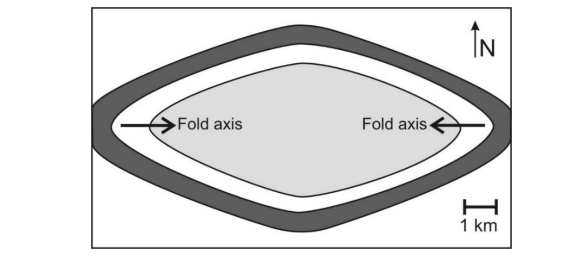
\includegraphics[width=0.6\textwidth]{figs/fig6.png}
    \caption{Image for questions 45}
    \label{fig:question45}
\end{figure}
\vspace{0.5cm}




\begin{enumerate}
\item antiform with axial culmination.
\item horizontal fold.
\item plunging antiform.
\item synform with axial depression.
\end{enumerate}
\vspace{0.5cm}


\item Match the following fossil taxa in Group I with their corresponding features in Group II:

\begin{multicols}{2}
\textbf{Group I}
\begin{flushleft}
P. Bryozoa\\
Q. Ostracoda\\
R. Foraminifera\\
S. Conodont
\end{flushleft}

\columnbreak

\textbf{Group II}
\begin{flushleft}
1. Denticles\\
2. Chamber\\
3. Carapace\\
4. Zooid
\end{flushleft}
\end{multicols}

\begin{enumerate}
\item P--4,\ Q--3,\ R--2,\ S--1
\item P--3,\ Q--4,\ R--2,\ S--1
\item P--4,\ Q--1,\ R--2,\ S--3
\item P--3,\ Q--1,\ R--4,\ S--2
\end{enumerate}
\vspace{0.5cm}

\item In the given schematic diagram, cross beds are exposed on a vertical rock face. The feature XY (bold line) represents a/an


\begin{figure}[H]
    \centering
    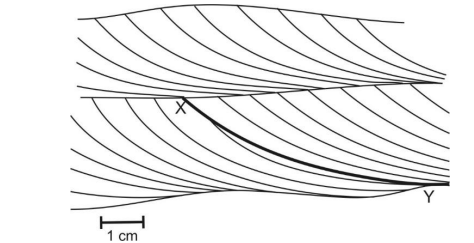
\includegraphics[width=0.6\textwidth]{figs/fig7.png}
    \caption{Image for questions 47}
    \label{fig:question47}
\end{figure}
\vspace{0.5cm}








\begin{enumerate}
\item reactivation surface.
\item foreset of cross bed.
\item scoured channel base.
\item angular unconformity.
\end{enumerate}
\vspace{0.5cm}

\item The schematic diagram represents thin section of a carbonate rock. The type of cement formed by large calcite crystals is known as

\begin{figure}[H]
    \centering
    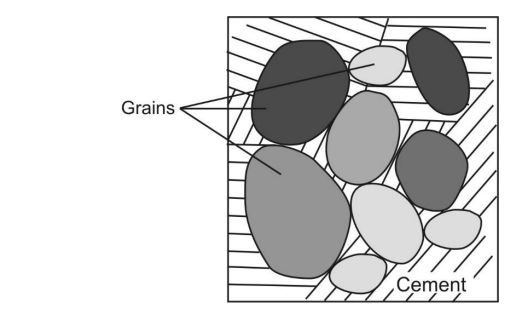
\includegraphics[width=0.6\textwidth]{figs/fig8.png}
    \caption{Image for questions 48}
    \label{fig:question48}
\end{figure}
\vspace{0.5cm}






\begin{enumerate}
\item overgrowth cement.
\item poikilotopic cement.
\item isopachous cement.
\item meniscus cement.
\end{enumerate}
\vspace{0.5cm}

\item Based on the three statements given below, choose the CORRECT option.\\
Statement I: Echinoids have water vascular system.\\
Statement II: Delthyrium and pedicle foramen are found in the brachial valve of brachiopods.\\
Statement III: Cardinal teeth, adductor muscles and chondrophore are found in bivalves.
\begin{enumerate}
\item Statements I and III are correct, statement II is incorrect.
\item Statements II and III are correct, statement I is incorrect.
\item Statements I and II are correct, statement III is incorrect.
\item Statements I, II and III are correct.
\end{enumerate}
\vspace{0.5cm}

\item The total number of symmetry elements in the crystal class represented by the point group 4/m32/m is
\begin{enumerate}
\item 21
\item 22
\item 23
\item 24
\end{enumerate}
\vspace{0.5cm}

\item The ratio of bridging to non--bridging oxygen atoms in the amphibole structure is
\begin{enumerate}
\item 4:11
\item 5:6
\item 2:7
\item 1:2
\end{enumerate}
\vspace{0.5cm}

\item Match the following basins in Group I with their corresponding formations in Group II:

\begin{multicols}{2}
\textbf{Group I}
\begin{flushleft}
P. Cauvery\\
Q. Damodar\\
R. Chhattisgarh\\
S. Indravati
\end{flushleft}

\columnbreak

\textbf{Group II}
\begin{flushleft}
1. Lohardih\\
2. Tiratgarh\\
3. Raniganj\\
4. Kallamedu
\end{flushleft}
\end{multicols}

\begin{enumerate}
\item P--4,\ Q--3,\ R--1,\ S--2
\item P--3,\ Q--4,\ R--2,\ S--1
\item P--4,\ Q--1,\ R--3,\ S--2
\item P--2,\ Q--3,\ R--1,\ S--4
\end{enumerate}
\vspace{0.5cm}

\item Based on the three statements given below, choose the CORRECT option.\\
Statement I: Gigantopithecus is a genus of the family Hominidae\\
Statement II: Equus is a living genus of the family Equidae\\
Statement III: Gomphotherium is a genus belonging to the order Proboscidea
\begin{enumerate}
\item Statements I and II are correct, statement III is incorrect.
\item Statements I and III are correct, statement II is incorrect.
\item Statements II and III are correct, statement I is incorrect.
\item Statements I, II and III are correct.
\end{enumerate}
\vspace{0.5cm}

\item In porphyry copper deposits, the order of alteration zones from the intrusive body outwards is
\begin{enumerate}
\item propylitic $\rightarrow$ argillic $\rightarrow$ phyllic $\rightarrow$ potassic
\item argillic $\rightarrow$ phyllic $\rightarrow$ potassic $\rightarrow$ propylitic
\item potassic $\rightarrow$ phyllic $\rightarrow$ argillic $\rightarrow$ propylitic
\item potassic $\rightarrow$ argillic $\rightarrow$ phyllic $\rightarrow$ propylitic
\end{enumerate}
\vspace{0.5cm}

\item Which is the CORRECT sequence of ore minerals in their increasing order of reflectance?
\begin{enumerate}
\item Galena, Sphalerite, Magnetite, Pyrite
\item Magnetite, Sphalerite, Galena, Pyrite
\item Sphalerite, Magnetite, Galena, Pyrite
\item Galena, Magnetite, Sphalerite, Pyrite
\end{enumerate}
\vspace{0.5cm}


\item Which of the following stratigraphic successions is/are arranged in CORRECT chronological order?
\begin{enumerate}
\item Muth Quartzite -- Syringothyris Limestone -- Fenestella Shale -- Panjal Volcanics
\item Barakar Formation -- Bijori Formation -- Pachmarhi Formation -- Bagra Formation
\item Chiravati Group -- Papaghni Group -- Nallamalai Group -- Kurnool Group
\item Kaimur Group -- Semri Group -- Bhander Group -- Rewa Group
\end{enumerate}
\vspace{0.5cm}

\item Which of the following options represent(s) simultaneous crystallization of two minerals in the given feature(s)?
\begin{enumerate}
\item Granophyric texture
\item Myrmekite
\item Corona of orthopyroxene around anhedral olivine
\item Cumulate pyroxene with interstitial plagioclase
\end{enumerate}
\vspace{0.5cm}

\item Which of the following textures suggest(s) post--kinematic growth of the mentioned mineral?
\begin{enumerate}
\item Randomly oriented chlorite grain aggregates pseudomorphing porphyroblast
\item Garnet porphyroblast wrapped by external foliation
\item Foliation defining biotite wrapping around a porphyroblast
\item Porphyroblastic garnet containing helicitic fold as internal schistosity
\end{enumerate}
\vspace{0.5cm}

\item In the schematic cross--section of a hill, a planar discontinuity intersects a planar slope face. Using kinematic analysis, which of the following conditions favor(s) plane failure to occur?

\begin{figure}[H]
    \centering
    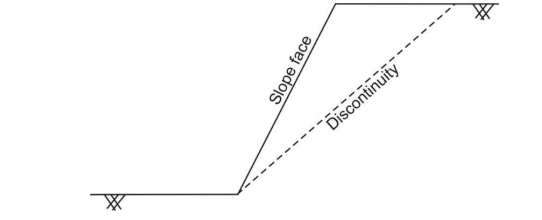
\includegraphics[width=0.6\textwidth]{figs/fig9.png}
    \caption{Image for questions 59}
    \label{fig:question59}
\end{figure}
\vspace{0.5cm}




\begin{enumerate}
\item The dip of the discontinuity surface is less than that of the slope face.
\item Friction angle on the discontinuity surface is more than the dip of the slope face.
\item Friction angle on the discontinuity surface is less than the dip of the discontinuity.
\item The dip direction of the discontinuity surface is same as that of the slope face.
\end{enumerate}
\vspace{0.5cm}

\item In a drainage basin, the number of the 1st, 2nd, 3rd, 4th and 5th order streams are 240, 40, 8, 2 and 1, respectively. The average of all calculated bifurcation ratios is \underline{\hspace{10mm}}.  
\vspace{0.5cm}

\item A sandstone follows Mohr--Coulomb failure criterion. If the uniaxial compressive strength and the angle of the internal friction of the sandstone are 7 MPa and 30$^\circ$, respectively, the calculated cohesion of the rock is \underline{\hspace{10mm}} MPa.  
\vspace{0.5cm}

\item At a certain depth in the crust, the maximum and minimum principal compressive stresses are 150 MPa and 75 MPa, respectively, which lead to normal faulting. If the average density of the crust is 2700 kg/m$^3$, the crustal depth of fracture initiation according to Anderson's theory of faulting is \underline{\hspace{10mm}} km. (g = 10 m/s$^2$)  
\vspace{0.5cm}

\item A cylindrical soil sample of 10 cm diameter is tested in a constant--head permeameter. A volume of 250 cm$^3$ of water is collected in 5 minutes when the constant--head difference between tapping points 15 cm apart is 5 cm. Considering Darcy flow, the absolute value of coefficient of permeability in cm/s is \underline{\hspace{10mm}}. ($\pi$ = 3.14)  
\vspace{0.5cm}

\item The minimum anion--to--cation radius ratio at which a 3--fold coordination becomes possible is \underline{\hspace{10mm}}.  
\vspace{0.5cm}

\item The mole fraction of jadeite in the pyroxene of composition {\small(Ca$_{0.667}$Na$_{0.333}$Fe$^{2+}_{0.121}$Fe$^{3+}_{0.125}$Mg$_{0.546}$Al$_{0.208}$)Si$_2$O$_6$} is \underline{\hspace{10mm}}.
\vspace{0.5cm}

\vspace{0.5cm}













































































































\end{enumerate}
\end{document}
